Previous sections have outlined the importance of PSCs to improve the accesibility and other issues in 
the e-Procurement sector. The applicability of semantic technologies and Linked Data has been also presented 
as a method to improve interoperability and integration among systems. Furthermore the MOLDEAS lifecycle has been 
also outlined as well as existing conversion methods and common features of PSCs. In order to carry out 
the promotion of PSCs to Linked Data following this lifecycle, a detailed summary of the main tasks is presented below.

\begin{itemize}
 \item  Firstly, the criteria to select and promote PSCs, see Table~\ref{table:pscs-ld}, are presented:
\begin{itemize}
 \item The use of the CPV 2008 is mandatory for all public procurement notices according 
 to the Regulation (EC) Nº 2195/2002 of the European Parliament and it is used as a hub classification.
 \item European classifications such as CPC or CPA have direct mappings (hand-made) to the CPV so they perfectly fit 
 to the task $t_8$ of interlinking RDF resources (the SKOS property \texttt{skos:exactMatch} can be used for this purpose).
 \item International classifications such as ISIC, SITC or NAICS enable the interoperability with 
 other e-Procurement and e-Commerce systems as well as activities in the field of statistics.
 \item GoodRelations and Product Ontology (PO) are two of the main references in the e-Commerce sector. 
 That is why we reuse their definitions and instances with the objective of aligning the linkage of PSCs to existing efforts. 
 \item Other classifications such as TARIC, UNSPSC, PRODCOM or NAPCS are ongoing work and they will be also linked to the CPV.
\end{itemize}

\begin{table}[!ht]
\renewcommand{\arraystretch}{1.3}
\begin{center}
\begin{tabular}[c]{|p{6cm}|l|p{6cm}|} 
\hline
  \textbf{PSC} &  \textbf{Acronym} & \textbf{Source} \\\hline
  Common Procurement Vocabulary, (2003 and 2008) & CPV & European Union \\ \hline
  Combined Nomenclature 2012 & CN & European Union \\ \hline
  Central Product Classification, version 2 (2008) & CPC & European Union \\ \hline
  Product Classification by Activity (2008) & CPA & European Union \\ \hline
  International Standard Industrial Classification of All Economic Activities, Rev.4 & ISIC & United Nations Statistics Division \\ \hline
  North American Industry Classification System 2007 y 2012 & NAICS & United States \\ \hline
  Standard International Trade Classification, Revision 4 & SITC & United Nations Statistics Division \\ \hline
%\textit{Nomenclature générale des activités économiques dans les Communautés européennes} & NACE & Unión Europea \\ \hline
\hline
\end{tabular}
\caption{Product Scheme Classifications.}\label{table:pscs-ld}
  \end{center}
\end{table} 

 \item Tasks $t_1$ and $t_5$. There is an implicit structure in each product classification 
 that enables the use of graph definitions (tree and forest), see Figure~\ref{fig:pscs-data-model}.
 \begin{itemize}
  \item Product categories. A PSC is divided into product categories, $Cat^k_{psc}$, that group different elements according to 
  hierarchy levels generating a disjointed set of elements. Thus, each PSC element or term is defined in only one $Cat^k_{psc}$.
  \item Taxonomy. Apart from categories and hierarchy division, each product sector can be considered as a tree, $T_{psc}$, 
  and the whole set of trees builds a forest, $F_{psc}$. Each $t^0_{psc}$ element is the root of a product sector, each $t_{psc}$ 
  is part of only one $T_{psc}$ and the set product sectors are also disjointed by the forest definition.
 \end{itemize}
 
 The use of the SKOS Core Recommendation to model PSCs is then justified due to the fact this ontology is based on two 
 main classes \texttt{skos:Concept} and \texttt{skos:ConceptScheme}. Thus all PSC elements are 
 an instance of the class \texttt{skos:Concept}. Therefore the interpreation of each element $t_{psc}$ 
 is obvious and avoids the issues presented in Section~\ref{sect:least} keeping all original PSC semantics. In order 
 to group all PSC elements under a common concept, a new class $PSCConcept$ is defined as subclass of 
 \texttt{skos:Concept}. Furthermore this class can be divided into different categories to represent 
 the conceptual hierarchy of the PSC, if any. Thus for each $Cat_{psc}^k$ a subclass of $PSCConcept$ can be defined, e.g. 
 Equation~\ref{cpv-st} represents the CPV structure.
 
 \begin{equation}\label{cpv-st}
 \begin{split}
 PSCConcept\ \equiv Division\ \sqcup\ Group \sqcup\ Class \sqcup\ Category \\
 Division \sqcap\ Group \sqcap\ Class\ \sqcap\ Category = \perp
 \end{split}
\end{equation}

  As Section~\ref{sect:least} has outlined, the PSC taxonomy should not be interpreted as a classical \texttt{is-a} hierarchy but 
  the SKOS Core ontology defines specific properties such as \texttt{skos:inScheme}, \texttt{skos:related}, \texttt{skos:broader Transitive} or
  \texttt{skos:narrowerTransitive} that perfectly match the requirements of establishing relationships among PSC elements. Finally an 
  instance of a ``semantized'' PSC element, $t_{psc}$, is presented in Table~\ref{table:properties}. 
  
 \begin{figure}[!ht]
\centering
	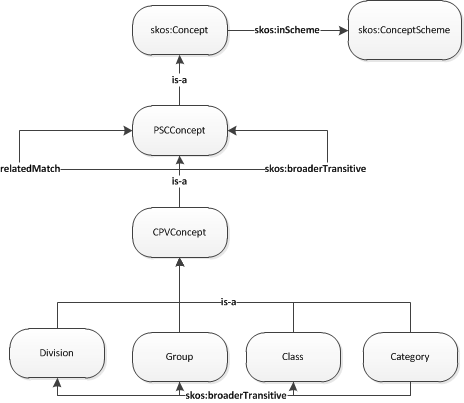
\includegraphics[width=\textwidth]{./imgs/fig-2}
 \caption{A partial view of the data model for PSCs in SKOS.}
 \label{fig:pscs-data-model}
\end{figure}

 \begin{table}[!ht]
\renewcommand{\arraystretch}{1.3}
\begin{center}
\begin{tabular}[c]{|p{3.55cm}|p{5.5cm}|p{5cm}|} 
\hline
  \textbf{Property} &  \textbf{Description} & \textbf{Example} \\\hline
  \texttt{rdf:type} & Type of a PSC element $t_{psc}$ & a \texttt{gr:ProductOr ServiceModel}, \texttt{PSCConcept} \\ \hline
  \texttt{skos:inScheme} & URI to the PSC dataset $T_{psc}$ & \texttt{skos:inScheme} cpv2008:ds \\ \hline
  \texttt{dct:identifier} & Id used in the URI of the element $t_{psc}$ &  \texttt{dc:identifier} "30210000"$\textasciicircum\textasciicircum$xsd:string \\ \hline
  \texttt{dct:subject} & Original Id of the element $t_{psc}$ &  \texttt{dc:subject} "30210000-4"$\textasciicircum\textasciicircum$xsd:string \\ \hline
  \texttt{skos:closeMatch} and \texttt{pscs:relatedMatch} & URI to a target PSC element $t'_{psc}$ that is partially related to a source PSC element $t_{psc}$ & \texttt{po:machine} \\ \hline
  \texttt{skos:exactMatch} & URI to a target PSC element $t'_{psc}$ that is related to a source PSC element $t_{psc}$ & \texttt{cpv2003:30216000} \\ \hline
  \texttt{pscs:level} & Level in the hierarchy of an element $t_{psc}$ when an explicit hierarchy definition is missing & \texttt{pscs:level} ``5'' \\ \hline  
  \texttt{skos:broader Transitive} & URI to a PSC element $t'_{psc}$ ancestor of a broader PSC element $t_{psc}$ & \texttt{skos:broaderTransitive} cpv2008:30200000 \\ \hline
  \texttt{skos:prefLabel} & Multilingual labels and descriptions &  "Data-processing machines (hardware)"@EN \\ \hline
\hline
\end{tabular}
\caption{Main semantic properties used for describing a PSC element.}\label{table:properties} 
  \end{center}
\end{table} 


\item Task $t_3$. The Linked Data community has released a lot of vocabularies to model information and 
knowledge in different domains. One of the keypoints to improve interoperability among sytems 
keeping semantics and, therefore, reasoning capabilities lies in the reuse of these definitions. That is 
why some existing vocabularies have been selected, see Table~\ref{table:vocabs}, to model the PSCs.


 \begin{table}[!ht]
\renewcommand{\arraystretch}{1.3}
\begin{center}
\begin{tabular}[c]{|l|p{8cm}|} 
\hline
  \textbf{Vocabulary prefix} &  \textbf{Description} \\\hline
 dbpedia &  Reuse of DBPedia concepts and properties \\ \hline 
 dc and dct & Dubling Core properties for describing metadata \\ \hline  
 gr & Use of the GoodRelations vocabulary to describe products and services \\\hline 
 po & Use of the ProductOntology vocabulary to create links to existing product and service definitions\\\hline 
 skos & Taxonomy specification and labeling properties \\ \hline
 void & Description of datasets metadata \\\hline
\hline
\end{tabular}
\caption{Main semantic vocabularies selected to model a PSC. These prefixes have been retrieved using the ``Prefix.cc'' service.}\label{table:vocabs} 
  \end{center}
\end{table} 


\item Task $t_6$. In order to get a successful promotion of raw data, the design of a good URI Scheme 
is a key-task~\cite{Heath_Bizer_2011}. Table~\ref{table:pscs-uri} presents the PSCs URI scheme with the aim of addressing the desired features 
of providing ``Cool Uris'', keep the namespaces under our control, etc. and easing the reuse of RDF resources in the ``Web of Data''.
  
 \begin{table}[!ht]
\renewcommand{\arraystretch}{1.3}
\begin{center}
\begin{tabular}[c]{|p{5cm}|p{4.5cm}|p{5cm}|} 
\hline
  \textbf{URI} &  \textbf{Description} & \textbf{Example} \\\hline
  \url{http://purl.org/weso/pscs/} & URI base: <base\_uri> & NA \\ \hline
  \url{<base_uri>/ontology} & Common definitions & \url{<base_uri>/ontology/PSCConcept} \\ \hline
  \url{<base_uri>/resource/ds} & Description of the PSCs Catalogue & \url{<base_uri>/resource/ds} \\ \hline
  \url{<base_uri>/{psc}/{version|year}} & PSC Namespace & \url{<base_uri>/cpv/2008} \\ \hline
  \url{<base_uri>/{psc}/{version|year}/ontology} & Specific definitions & \url{<base_uri>/cpv/2008/ontology} \\ \hline
  \url{<base_uri>/resource/{psc}/{version|year}/{id}} & URI for RDF resources & \url{<base_uri>/cpv/2008/resource/30210000} \\ \hline
  \url{<base_uri>/resource/{psc}/{version|year}/ds} & Description of the PSC dataset  & \url{<base_uri>/cpv/2008/resource/ds} \\ \hline
\hline
\end{tabular}
\caption{Design of an URI Scheme for the PSCs Catalogue.}\label{table:pscs-uri}
  \end{center}
\end{table} 

\item Task $t_8$. The broad aim of this task is to enable the possibility of querying, 
public procurement notices from any PSC. The mappings can be generated following two approaches: 
1) exact mappings created by a domain expert or 2) related, through the execution of a custom entity reconciliation process 
based on NLP techniques. To do so a PSC reconciliation service has been designed using the Apache Lucene and Solr libraries in which
both filters and the syntactic search engine can be easily customized. Firstly a target PSC is selected and their descriptors (in English) 
are indexed using Apache Lucene. After that the mappings between elements in a source PSC are automatically discoverd and generated through the execution 
of queries against the indexed PSC. Basically the creation of a mapping lies in a string comparison between the source descriptor and the 
target descriptor. Nevertheless the personalization of Apache Lucene and Solr allows us the creation of more accurate mappings.

\item Task $t_9$. Since a model for representing PSCs is available the real transformation to RDF has been performed using Google Refine 
and a Java processor. The results of promoting to RDF the selected PSCs are presented in Table~\ref{ganancia-terminos}, 
more specifically the first four columns specify respectively the vocabulary of a PSC ($V_{psc}$), the number of elements 
to be promoted (\#$V_{psc}$), the number of generated RDF triples and the number of links to the CPV 2008. 
Thus we have promoted more than $42035$ product descriptions, generating more than $1842053$ triples and creating $21715$ 
links among them. 

Finally, Figure~\ref{fig:example-cpv-code} shows a partial example of a generated RDF resource in which multilinguism features, 
hierarchy relationships and links can be found. Furthermore, data can be now exploited through SPARQL queries 
such as ``Give me 100 products or services related to construction in any PSC that have a mapping with products or 
services in CPV (descriptions in English)'', see Figure~\ref{fig:example-sparql-query}, using more descriptors and 
different vocabularies.

\item Other tasks such as ``Add metainformation'' are considered optional but relevant to mainly ease the process of dataset discovery.

\item Task $t_{14}$. Once the PSCs are available as RDF is necessary to make them publicly available through a Linked Data infrastructure. To 
do so all RDF triples and the ontology have been deployed in a RDF repository (OpenLink Virtuoso), thus data can be accessed through 
a SPARQL endpoint. Furthermore and with the aim of making dereferenceable URIs and enabling content negotiation an instance 
of Pubby (a Linked Data frontend) has been also deployed. Besides in order to ease the creation and execution of SPARQL queries, SNORQL 
(a tool for exploring SPARQL endpoints) has been also released. Finally, the new PSCs catalogue has been released to the 
LOD community, added to the ``datahub.io'' register and joined the LOD Cloud Diagram under the dataset id ``\texttt{pscs-catalogue}''.

\item Task $t_{12}$. The MOLDEAS lifecycle purposes a validation method based on a checklist of $196$ points compiled from books, 
W3C specifications, Open Data and Linked Data principles, CKAN validator, LOD Cloud requirements, etc. which values can be 
``Applicable and positive (Yes)'', ``Applicable and not found (No)'' or ``Not Applicable (N/A)''. The objective of this questionnaire is 
to ensure the principles of the LOD initiative for easing the reuse, maintenance, governance, coverage and expressivity of data. In order to compare 
the new version of a PSCs catalogue to existing public versions, we have carried out this survey obtaining the next results, 
see Figure~\ref{fig:results-4}, in which ``Reference'' corresponds to the MOLDEAS lifecycle perfect evaluation, ``CSV/Excel'' to the official publicly 
available versions of PCSs and ``Third-parties service'' to those versions managed by non-official organizations. 

 \begin{figure}[!ht]
\centering
	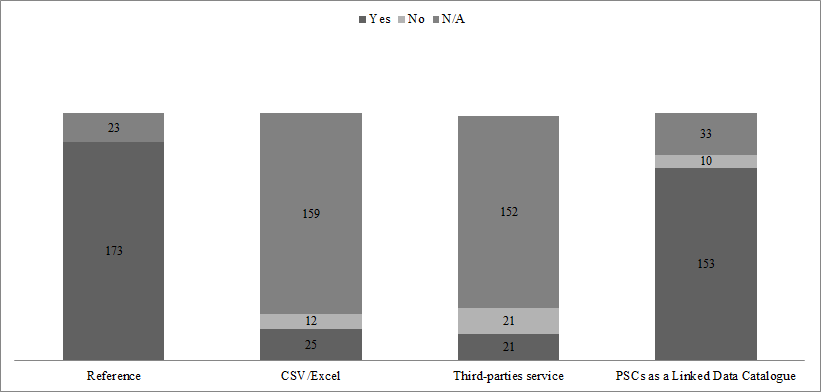
\includegraphics[width=12cm]{./imgs/fig-4}
 \caption{Validation and comparison of the PSCs Catalogue as Linked Data with regards to existing versions.}
 \label{fig:results-4}
\end{figure}



\end{itemize}



\begin{figure}[!ht]
\begin{lstlisting}[language=SQL,basicstyle=\ttfamily\scriptsize]  
cpv2008-res:30210000 a gr:ProductOrServiceModel, cpv-onto:Group;
  skos:prefLabel, gr:description, rdfs:label 	
  "Data-processing machines (hardware)"@EN ,
  "Naprave za obdelavo podatkov (strojna oprema)"@SL , 
  "Databehandlingsmaskiner (hardware)"@DA ,
  "Macchine per l'elaborazione di dati (hardware)"@IT ,
  "Databehandlingsmaskiner (maskinvara)"@SV ,
  "Maşini de procesare a datelor (hardware)"@RO ,   
  "Machines voor dataprocessing (hardware)"@NL , 
  ... ;
  dct:identifier "30210000"^^xsd:string;
  dct:subject "30210000-4"^^xsd:string;
  pscs-onto:relatedMatch   
    <http://www.productontology.org/id/dataprocessing>,
    <http://www.productontology.org/id/hardware> ,
    <http://www.productontology.org/id/machine> ;	
  skos:broaderTransitive cpv2008-res:30200000;
  skos:exactMatch 
    cpv2003-res:30216000, cpv2003-res:30215000,  cpv2003-res:30213000,   
    cpv2003-res:30212000, cpv2003-res:30211000,  cpv2003-res:30214000.
\end{lstlisting}
\caption{Partial example of CPV 2008 item in RDF.}
 \label{fig:example-cpv-code}
\end{figure}


\begin{figure}[!ht]
\begin{lstlisting}[language=SQL,basicstyle=\ttfamily\scriptsize]  
SELECT DISTINCT * WHERE{
   ?product pscs:relatedMatch 
    <http://www.productontology.org/id/construction> .
   ?product skos:closeMatch ?cpv .
   ?product skos:prefLabel ?productLabel .
   ?cpv skos:prefLabel ?cpvLabel .
   ?product skos:inScheme ?scheme .
   FILTER (?scheme != <http://purl.org/weso/pscs/cpv/2008/resource/ds>) .
   FILTER (lang (?cpvLabel) ="en" )
} LIMIT 100
\end{lstlisting}
\caption{Example of SPARQL query.}
 \label{fig:example-sparql-query}
\end{figure}


